\documentclass[UTF8,12pt,a4paper]{ctexart}
\usepackage[a4paper,margin=2.35cm,headheight=15pt]{geometry}
\usepackage{amsmath,amssymb,bm}
\usepackage{booktabs,array,tabularx,longtable}
\usepackage{graphicx,float,caption,subcaption}
\usepackage{xcolor,tikz}
\usepackage{hyperref}
\usepackage{siunitx}
\usetikzlibrary{arrows.meta,positioning,calc,fit}

\definecolor{navy}{HTML}{153A5B}
\definecolor{blue}{HTML}{2E75B6}
\definecolor{lightblue}{HTML}{EAF2F8}
\definecolor{green}{HTML}{2E7D5B}
\definecolor{orange}{HTML}{C76A20}
\definecolor{graytext}{HTML}{4B5563}

\hypersetup{colorlinks=true,linkcolor=navy,urlcolor=blue,citecolor=navy}
\pagestyle{plain}
\setlength{\parindent}{2em}
\setlength{\parskip}{0.32em}
\setlength{\emergencystretch}{2em}
\captionsetup{font=small,labelfont=bf}
\sisetup{detect-all}


\newcommand{\Yp}{\bm{Y}_{\mathrm{port}}}
\newcommand{\Yn}{\bm{Y}_{N}}
\newcommand{\Zb}{\bm{Z}_{b}}
\newcommand{\Cmat}{\bm{C}}
\newcommand{\Gmat}{\bm{G}}
\newcommand{\Rmat}{\bm{R}}
\newcommand{\Lmat}{\bm{L}}
\newcommand{\Gam}{\bm{\Gamma}}

\begin{document}

\begin{titlepage}
\centering
\vspace*{2.0cm}
{\Huge\bfseries\color{navy} 分段梯形网络高频变压器\\[0.35em]
矩阵建模、Simscape实现与双端口验证\par}
\vspace{1.2cm}
{\Large 实验十一详细技术报告\par}
\vspace{1.5cm}
\begin{tikzpicture}[node distance=1.1cm,>=Latex,scale=0.78,transform shape]
\node[draw=blue,rounded corners,fill=lightblue,minimum width=3.2cm,minimum height=1.0cm] (geo) {分段物理结构};
\node[draw=blue,rounded corners,fill=lightblue,right=of geo,minimum width=3.2cm,minimum height=1.0cm] (mat) {矩阵网络模型};
\node[draw=blue,rounded corners,fill=lightblue,right=of mat,minimum width=3.2cm,minimum height=1.0cm] (sim) {Simscape 独立实现};
\node[draw=green,rounded corners,fill=green!8,right=of sim,minimum width=3.2cm,minimum height=1.0cm] (val) {双端口一致性验证};
\draw[->,thick] (geo)--(mat);
\draw[->,thick] (mat)--(sim);
\draw[->,thick] (sim)--(val);
\end{tikzpicture}
\vfill
\begin{tabular}{rl}
\textbf{研究对象：} & 原、副边各四段的高频变压器梯形网络\\
\textbf{验证软件：} & MATLAB/Simulink/Simscape R2021b\\
\textbf{验证频段：} & \SI{1}{kHz}--\SI{10}{MHz}\\
\textbf{报告日期：} & 2026年7月28日
\end{tabular}
\vfill
{\large 本报告对应可复现实验文件与编译结果，不包含实物样机结论。}
\end{titlepage}

\begin{abstract}
本实验把传统连续式绕组梯形等效网络的“分段、组装、端口消元”思想迁移到高频变压器，建立了原、副边各四段、包含全耦合电感矩阵、纵向电容、节点对地电容以及逐段绕组间电容的宽频小信号模型。首先从支路--节点关联矩阵出发推导完整节点导纳矩阵，并通过Kron消元得到DAB可观测的二端口导纳矩阵。随后在Simscape中用自定义八绕组耦合元件和显式电压测试端口建立独立物理网络，对模型进行线性化，获得82阶状态空间模型。最终在161个对数频点上比较Simscape线性化结果与矩阵参考解。

验证结果表明，\SI{1}{kHz}--\SI{10}{MHz}范围内二者平均Frobenius相对误差为
\(2.016\times10^{-9}\)，最大误差为\(2.009\times10^{-8}\)；Simscape结果的最大互易性残差为
\(4.657\times10^{-10}\,\mathrm{S}\)。这证明当前拓扑组装、参数映射、端口定义和线性化链路在数值层面一致。需要强调的是，本结果属于“独立求解器、相同参数与相同模型结构”的实现验证，尚不能替代高频变压器样机、有限元或DAB开关运行验证。
\end{abstract}

\tableofcontents
\newpage

\section{实验目的与研究定位}

\subsection{为什么要把高频变压器分成梯形单元}
当前已有的三电容或低阶二端口模型适合辨识总漏感和总绕组间电容，但它把高频变压器作为一个整体，只能得到
\[
L_{\sigma},\quad C_{ps},\quad C_p,\quad C_s
\]
等终端等效量，无法回答“哪一段绕组的耦合发生了变化”。任富强相关工作的关键启发不是直接照搬普通电力变压器参数，而是保留以下建模思想：
\[
\text{结构分段}\rightarrow
\text{支路/节点矩阵组装}\rightarrow
\text{端口频响}\rightarrow
\text{局部参数反演}.
\]
本实验将这一思想改造成高频变压器版本，使每个分段均具有明确的电阻、电感、纵向电容、对地电容和绕组间电容，并让所有分段通过互感矩阵耦合。

\subsection{本次验证回答什么问题}
本次验证只回答三个基础问题：
\begin{enumerate}
  \item 数学矩阵模型是否按预期组装，且满足互易性、无源性和KCL；
  \item 同一物理网络在Simscape中能否编译、仿真和线性化；
  \item 两条独立实现链得到的二端口导纳是否一致。
\end{enumerate}

它尚不回答局部故障能否在真实DAB上可靠定位，也不证明分段电容变化与某一种绝缘老化存在唯一对应关系。

\section{四分段高频变压器模型}

\subsection{拓扑与变量}
原边与副边各划分为\(n=4\)段，共有\(2n=8\)条绕组阻抗支路。保留八个非参考节点：
\[
\bm{u}=
[u_{p1},u_{p2},u_{p3},u_{p4},u_{s1},u_{s2},u_{s3},u_{s4}]^{\mathrm T}.
\]
每一侧的第\(k\)段连接相邻节点；第4段末端接公共参考点。端口取原边首端\(p1\)和副边首端\(s1\)。

每个分段包含：
\begin{itemize}
  \item 串联电阻\(R_i\)；
  \item 全矩阵耦合的自感/互感\(\Lmat\)；
  \item 与该绕组段并联的纵向电容\(C_{s,i}\)；
  \item 节点到参考结构的电容\(C_{g,i}\)；
  \item 原、副边对应分段节点之间的绕组间电容\(C_{ps,i}\)。
\end{itemize}

\begin{figure}[H]
\centering
\begin{tikzpicture}[scale=0.92,>=Latex,every node/.style={font=\small}]
  \foreach \x/\lab in {0/p_1,2/p_2,4/p_3,6/p_4}{
    \fill[blue] (\x,2) circle (2pt) node[above=3pt] {\(\lab\)};
  }
  \foreach \x/\lab in {0/s_1,2/s_2,4/s_3,6/s_4}{
    \fill[orange] (\x,-2) circle (2pt) node[below=3pt] {\(\lab\)};
  }
  \foreach \x in {0,2,4}{
    \draw[thick] (\x,2)--(\x+2,2) node[midway,above] {\(R_{p}+sL_{p}\)};
    \draw[thick] (\x,-2)--(\x+2,-2) node[midway,below] {\(R_{s}+sL_{s}\)};
  }
  \draw[thick] (6,2)--(7.2,2)--(7.2,0);
  \draw[thick] (6,-2)--(7.2,-2)--(7.2,0);
  \draw (7.2,0)--(7.2,-0.18); \draw (6.85,-0.18)--(7.55,-0.18);
  \draw (6.95,-0.35)--(7.45,-0.35); \draw (7.05,-0.5)--(7.35,-0.5);
  \foreach \x in {0,2,4,6}{
    \draw[dashed,green!70!black] (\x,1.85)--(\x,-1.85)
      node[midway,right] {\(C_{ps}\)};
  }
  \draw[->,very thick,blue] (-1,2)--(-0.1,2) node[midway,above] {\(i_1\)};
  \draw[->,very thick,orange] (-1,-2)--(-0.1,-2) node[midway,below] {\(i_2\)};
  \node[draw,rounded corners,align=left,anchor=west] at (8.2,0)
  {所有八条绕组支路\\由\(\Lmat\)全矩阵耦合；\\图中未展开\(C_s,C_g\)。};
\end{tikzpicture}
\caption{四分段高频变压器梯形网络的概念拓扑}
\label{fig:concept}
\end{figure}

\subsection{基线参数}
\begin{table}[H]
\centering
\caption{本次数值基线参数}
\begin{tabular}{lll}
\toprule
参数 & 数值 & 说明\\
\midrule
分段数 \(n\) & 4/侧 & 共8条耦合绕组支路\\
变比 \(a\) & 4 & 副边量按\(1/a\)磁势系数处理\\
原边总电阻 & \SI{0.18}{\ohm} & 各段均分\\
副边总电阻 & \(\SI{0.18}{\ohm}/a^2\) & 折算后一致\\
原边总漏感 & \SI{3.6}{\micro H} & 各段均分\\
副边总漏感 & \(\SI{3.6}{\micro H}/a^2\) & 各段均分\\
励磁电感 \(L_m\) & \SI{220}{\micro H} & 形成公共磁通秩一项\\
原边纵向电容 & \SI{72}{pF}/段 & 并联于每段绕组\\
副边纵向电容 & \SI{42}{pF}/段 & 并联于每段绕组\\
总 \(C_{ps}\) & \SI{28.36}{pF} & 四段均分\\
对地电容 \(C_g\) & 3.5--\SI{7}{pF}/节点 & 非均匀设置\\
\bottomrule
\end{tabular}
\end{table}

\section{矩阵算法的完整推导}

\subsection{支路--节点关联矩阵}
定义绕组支路电流\(\bm{i}_b\in\mathbb{C}^{8}\)，并用关联矩阵
\(\Gam\in\mathbb{R}^{8\times 8}\)描述支路端点。每行对应一条绕组支路，起点填\( +1 \)，终点填\(-1\)；若终点为参考点，则该行只保留起点的\( +1 \)。于是
\[
\bm{v}_b=\Gam\bm{u}.
\]
这里采用“关联矩阵行对应支路”的约定，因此与某些文献使用转置关联矩阵的记号不同；只要全篇保持一致，物理结果不变。

\subsection{耦合阻抗矩阵}
在频域\(s=j\omega\)下，
\[
\Zb(s)=\Rmat+s\Lmat,\qquad
\Rmat=\operatorname{diag}(R_1,\ldots,R_8).
\]
本次Simscape实现采用结构化、但与基线全矩阵完全等价的电感表达：
\[
\boxed{\Lmat=
\operatorname{diag}(\bm{L}_{\mathrm{leak}})
+L_c\bm{a}\bm{a}^{\mathrm T}},
\]
其中
\[
\bm{a}=[1,1,1,1,-1/a,-1/a,-1/a,-1/a]^{\mathrm T},
\qquad L_c=L_m/n^2.
\]
因此支路方程为
\[
\Gam\bm{u}=\Zb\bm{i}_b,
\qquad
\bm{i}_b=\Zb^{-1}\Gam\bm{u}.
\]
结构化表达使R2021b的Simscape编译器无需展开64个独立符号互感，同时数值上仍等于原始\(8\times8\)电感矩阵。

\subsection{电容矩阵的盖章规则}
连接节点\(r\)和\(q\)的电容\(C\)对节点电容矩阵的贡献为
\[
\Delta\Cmat=C(\bm{e}_r-\bm{e}_q)(\bm{e}_r-\bm{e}_q)^{\mathrm T}.
\]
连接节点\(r\)与参考点的电容只贡献
\[
\Delta\Cmat=C\bm{e}_r\bm{e}_r^{\mathrm T}.
\]
将纵向电容、节点对地电容和逐段\(C_{ps,i}\)全部盖章，可得对称半正定矩阵\(\Cmat\)。若加入介质损耗，则以\(\Gmat\)表示并联电导矩阵。

\subsection{完整节点导纳矩阵}
节点外部注入电流为
\[
\bm{i}_{\mathrm{ext}}
=\Gam^{\mathrm T}\bm{i}_b+(\Gmat+s\Cmat)\bm{u}.
\]
代入支路电流：
\[
\boxed{
\Yn(s)
=\Gam^{\mathrm T}
(\Rmat+s\Lmat)^{-1}\Gam
+\Gmat+s\Cmat
}.
\]
数值实现中不显式计算矩阵逆，而是求解线性方程
\[
(\Rmat+s\Lmat)\bm{X}=\Gam,
\qquad
\Yn=\Gam^{\mathrm T}\bm{X}+\Gmat+s\Cmat,
\]
以降低病态频点的数值误差。

\subsection{Kron消元得到可测二端口}
将节点分为端口节点\(p=\{p_1,s_1\}\)和内部节点\(i\)：
\[
\begin{bmatrix}\bm{i}_p\\\bm{0}\end{bmatrix}
=
\begin{bmatrix}
\bm{Y}_{pp}&\bm{Y}_{pi}\\
\bm{Y}_{ip}&\bm{Y}_{ii}
\end{bmatrix}
\begin{bmatrix}\bm{u}_p\\\bm{u}_i\end{bmatrix}.
\]
内部节点无外部注入，故
\[
\bm{u}_i=-\bm{Y}_{ii}^{-1}\bm{Y}_{ip}\bm{u}_p.
\]
端口导纳为Schur补：
\[
\boxed{
\Yp
=\bm{Y}_{pp}
-\bm{Y}_{pi}\bm{Y}_{ii}^{-1}\bm{Y}_{ip}
}.
\]
因此
\[
\begin{bmatrix}I_1\\I_2\end{bmatrix}
=
\begin{bmatrix}Y_{11}&Y_{12}\\Y_{21}&Y_{22}\end{bmatrix}
\begin{bmatrix}V_1\\V_2\end{bmatrix}.
\]
这一式是后续DAB多运行窗口辨识的接口：DAB不是为了检测额外添加的装置，而是高频变压器原本所处的运行系统；多个工况窗口用于使端口电压矩阵在数值上满秩。

\section{Simscape独立实现}

\subsection{自定义八绕组耦合元件}
自定义元件直接实现时域微分方程
\[
\bm{v}
=\Rmat\bm{i}
+\operatorname{diag}(\bm{L}_{\mathrm{leak}})\dot{\bm{i}}
+\bm{a}L_c\bm{a}^{\mathrm T}\dot{\bm{i}}.
\]
八对电气守恒端口分别连接各分段；纵向、对地和绕组间电容由标准Simscape电容元件独立搭建。模型参数写入模型工作区，避免依赖临时基础工作区。

\subsection{显式电压测试端口}
第一次线性化使用标准“受控电压源+电流传感器+转换器”，虽然模型可编译，但\texttt{linmod}得到的输出矩阵为零，导致四个导纳元素全为零。为排除转换链路盲区，新建电压测试端口，其方程为
\[
v_p-v_n=v_{\mathrm{cmd}},\qquad i_{\mathrm{meas}}=-i_{\mathrm{source}}.
\]
其中负号把“理想源内部由\(p\)流向\(n\)的电流”统一为“流入被测网络的端口电流”。这一符号修正具有清晰的诊断轨迹：
\[
\text{零输出}\rightarrow
\text{显式输出后误差恰为2}\rightarrow
\text{统一电流方向后误差降至}10^{-9}\text{量级}.
\]

\begin{figure}[H]
\centering
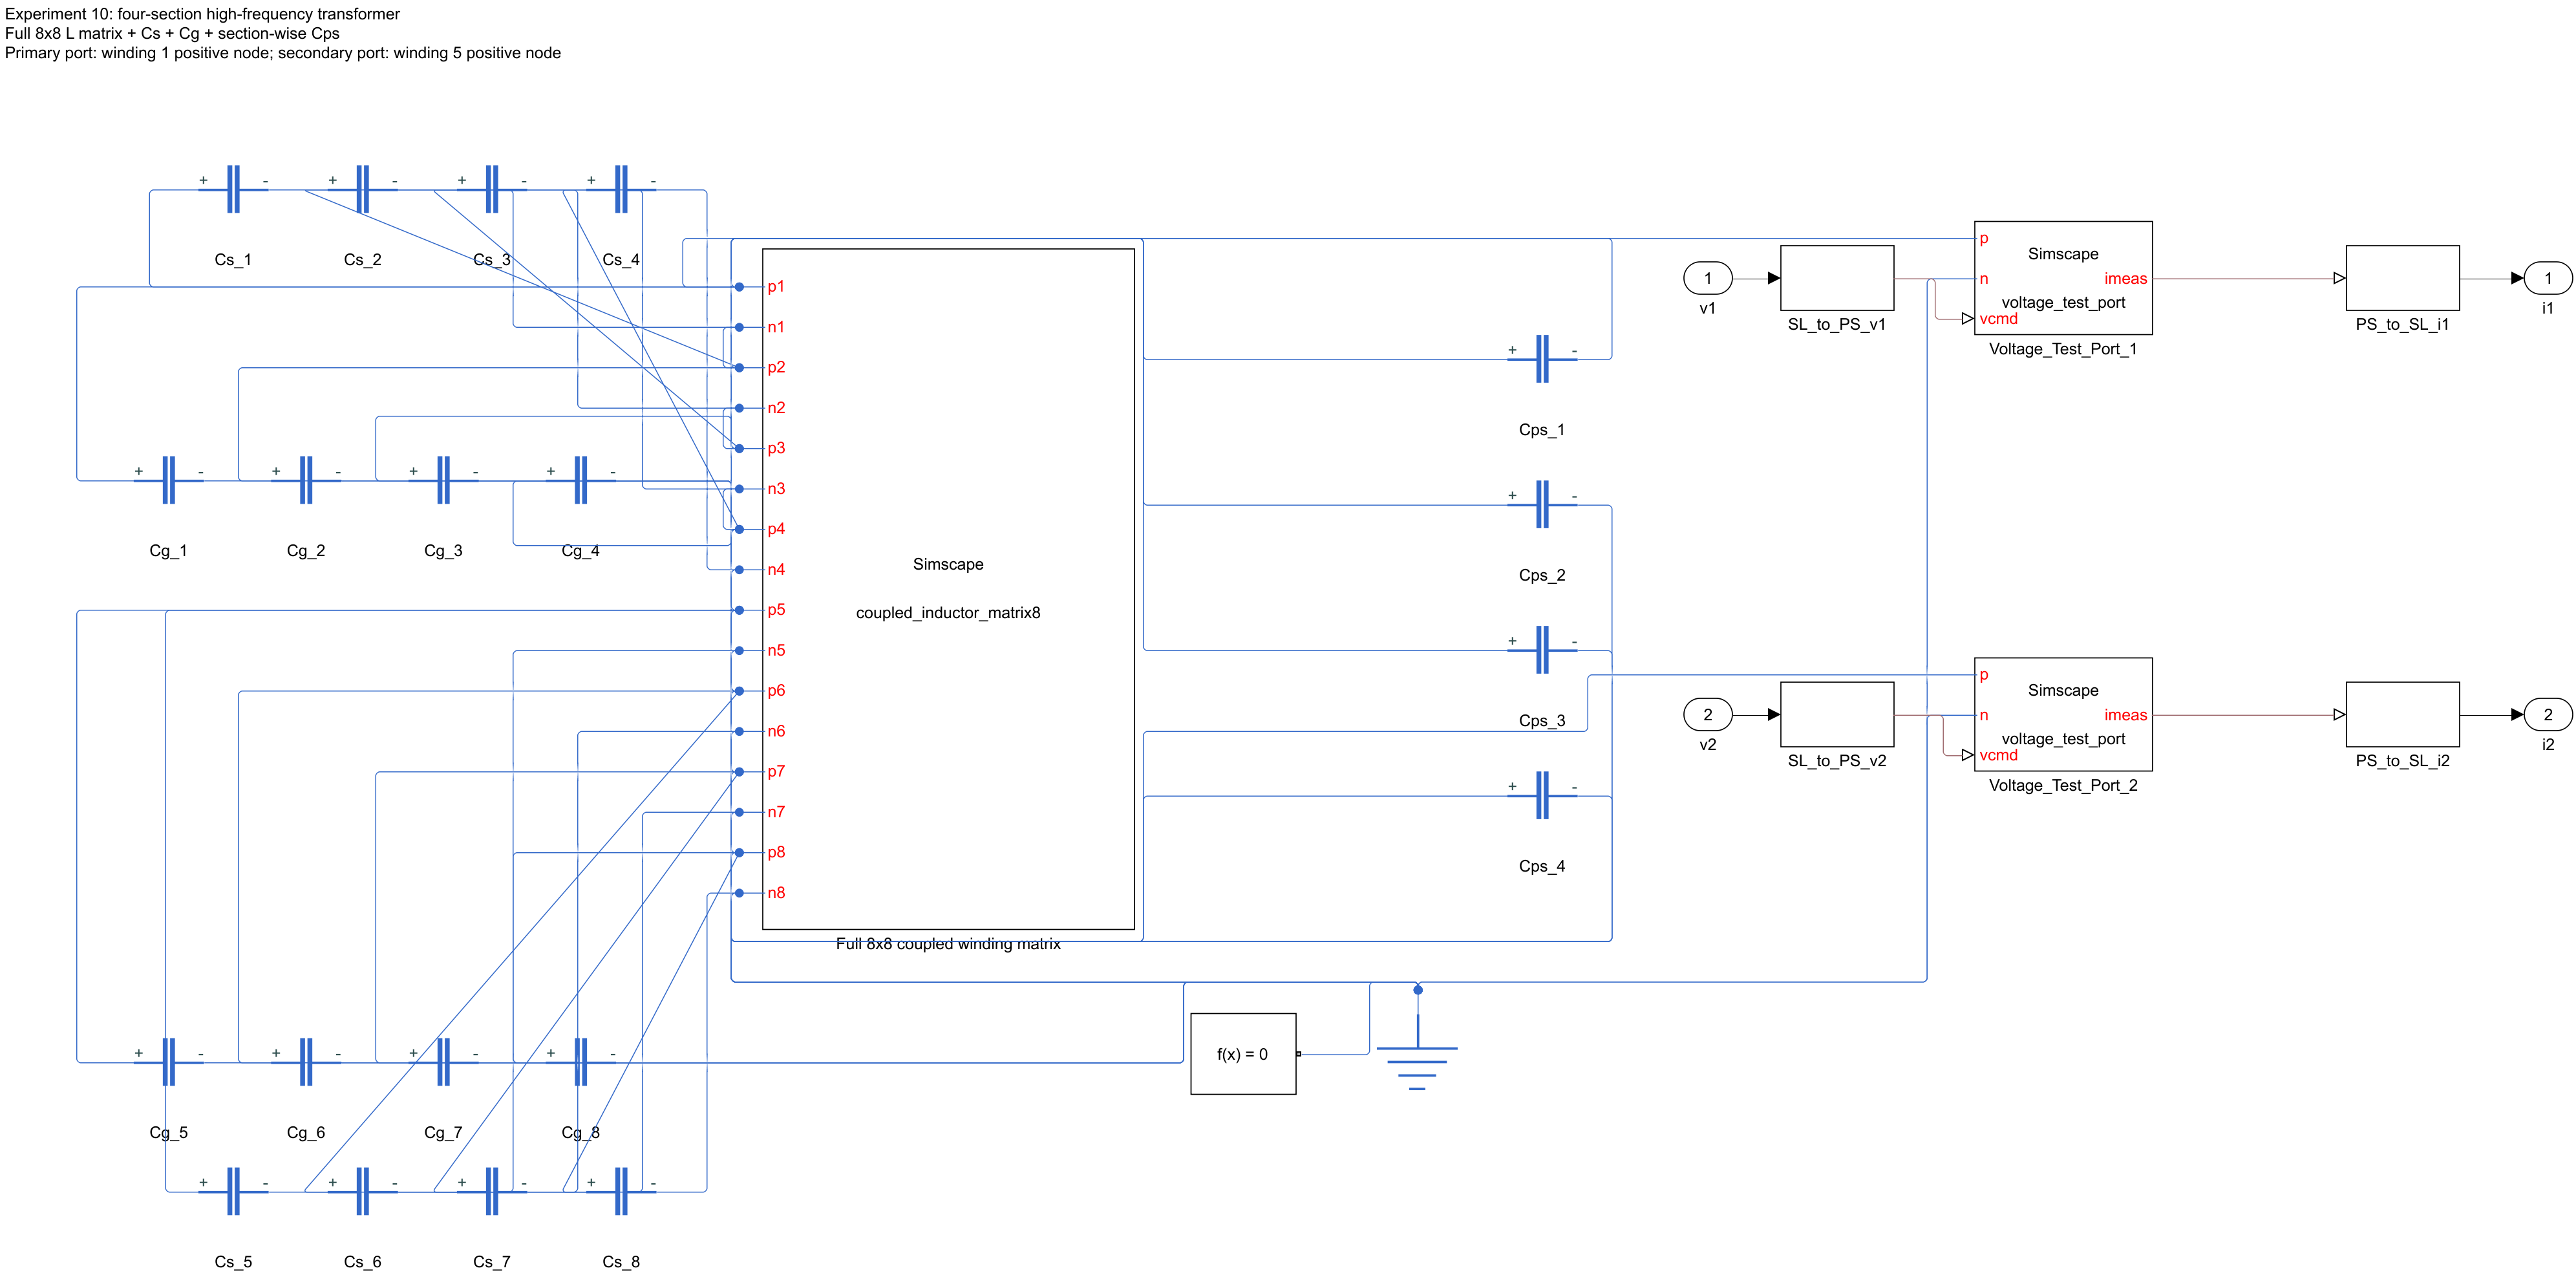
\includegraphics[width=\textwidth]{figures/simscape_model_overview.png}
\caption{实际生成的四分段Simscape双端口线性化模型}
\label{fig:simscape}
\end{figure}

\subsection{状态空间线性化}
Simscape网络在线性化后得到
\[
\dot{\bm{x}}=\bm{A}\bm{x}+\bm{B}\bm{v}_p,\qquad
\bm{i}_p=\bm{C}\bm{x}+\bm{D}\bm{v}_p.
\]
本次状态数为82。频域二端口导纳由
\[
\boxed{
\Yp^{\mathrm{SS}}(j\omega)
=\bm{C}(j\omega\bm{I}-\bm{A})^{-1}\bm{B}+\bm{D}
}
\]
计算。参考模型则直接按上一节的节点导纳和Kron消元求解，两条链路在元件实现和求解器层面相互独立。

\section{验证方案与判据}

\subsection{频率网格}
在
\[
f\in[\SI{1}{kHz},\SI{10}{MHz}]
\]
上选取161个对数等距频点，比较全部四个复导纳元素。

\subsection{误差与物理一致性指标}
第\(k\)个频点的整体相对误差定义为
\[
\varepsilon_F(f_k)
=
\frac{
\|\Yp^{\mathrm{SS}}(f_k)-\Yp^{\mathrm{M}}(f_k)\|_F
}{
\|\Yp^{\mathrm{M}}(f_k)\|_F
}.
\]
互易性残差定义为
\[
\varepsilon_{\mathrm{rec}}(f_k)
=|Y_{12}^{\mathrm{SS}}(f_k)-Y_{21}^{\mathrm{SS}}(f_k)|.
\]
矩阵基线还单独检查：
\[
\Lmat=\Lmat^{\mathrm T},\quad
\lambda_{\min}(\Lmat)>0,\quad
\Cmat=\Cmat^{\mathrm T},\quad
\lambda_{\min}(\Cmat)>0,
\]
以及内部节点KCL残差和Kron消元前后的端口电流一致性。

\section{验证结果}

\subsection{Simscape与矩阵参考解}
\begin{table}[H]
\centering
\caption{双端口一致性验证的核心结果}
\begin{tabular}{lr}
\toprule
指标 & 结果\\
\midrule
Simscape线性化状态数 & 82\\
验证频点数 & 161\\
平均Frobenius相对误差 & \(2.0157\times10^{-9}\)\\
中位Frobenius相对误差 & \(1.6962\times10^{-10}\)\\
最大Frobenius相对误差 & \(2.0095\times10^{-8}\)\\
最大互易性残差 & \(4.6566\times10^{-10}\,\mathrm{S}\)\\
\bottomrule
\end{tabular}
\end{table}

\begin{figure}[H]
\centering
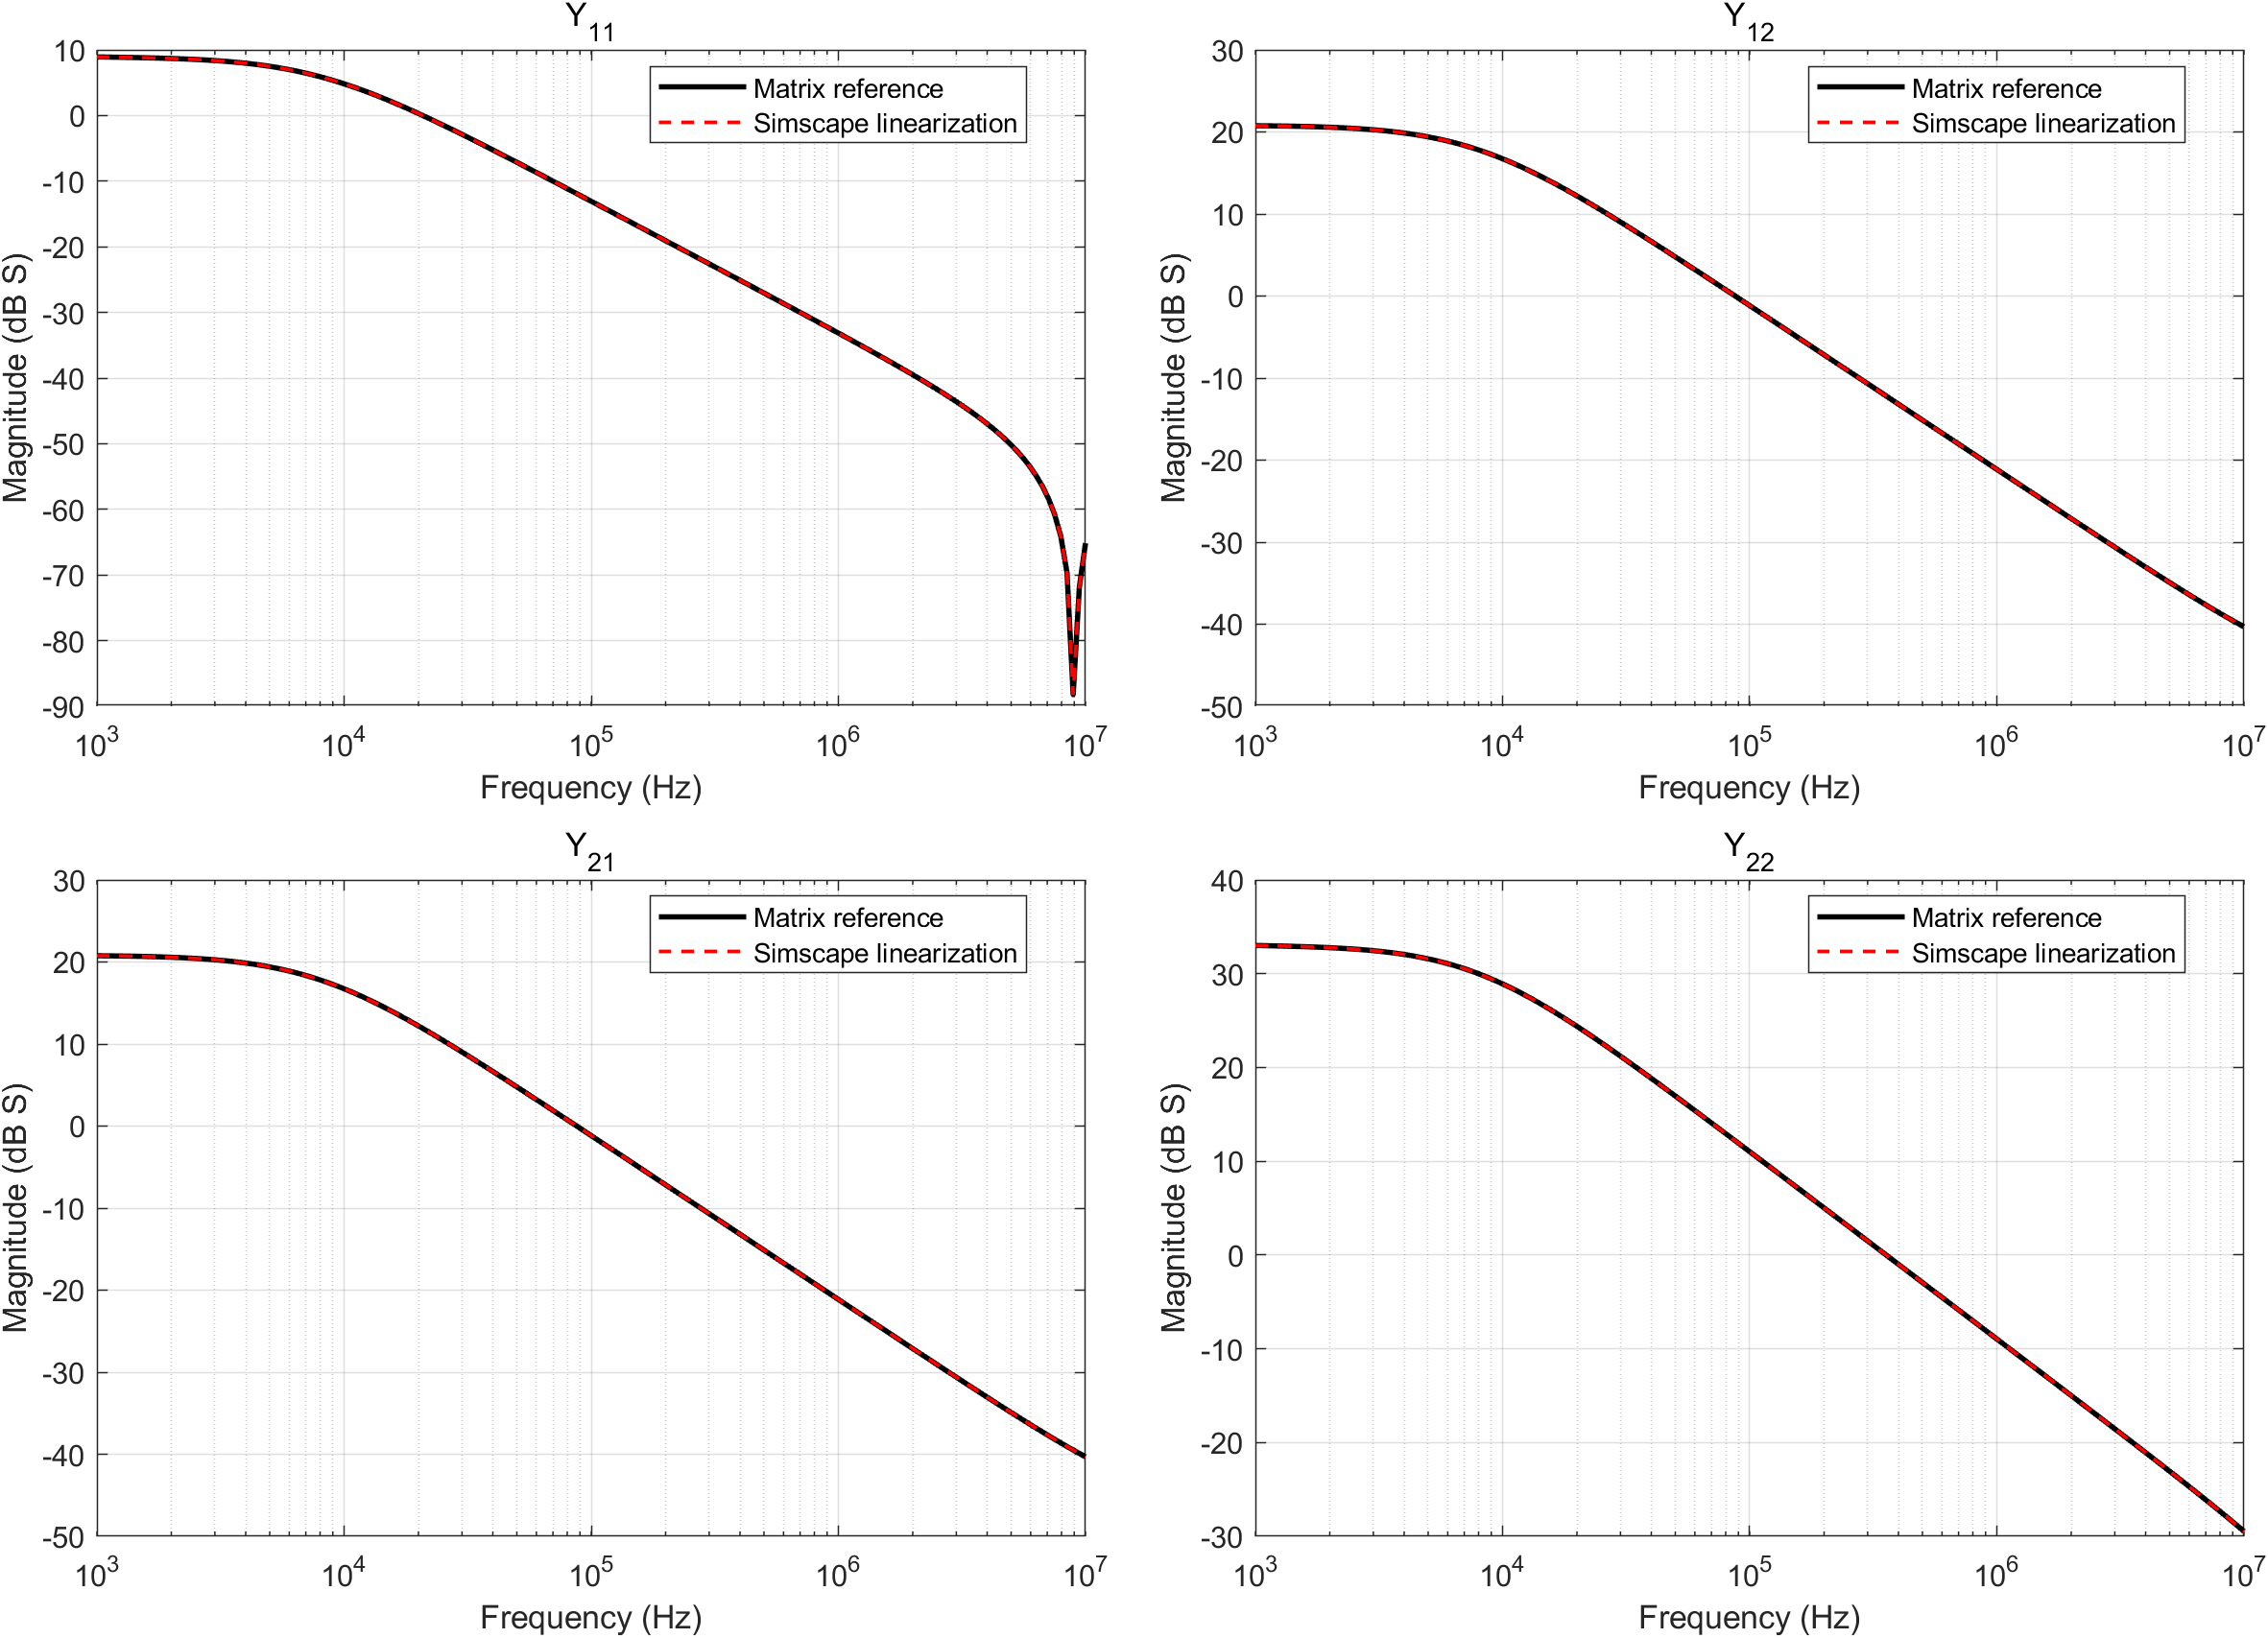
\includegraphics[width=\textwidth]{figures/simscape_vs_matrix_admittance.png}
\caption{矩阵参考解与Simscape线性化二端口导纳幅值对比。黑实线与红虚线在绘图分辨率内重合。}
\label{fig:validation}
\end{figure}

\subsection{矩阵基线的物理检查}
\begin{table}[H]
\centering
\caption{独立矩阵模型的结构性检查}
\begin{tabular}{lr}
\toprule
检查项 & 数值\\
\midrule
\(\Lmat\)对称残差 & \(0\)\\
\(\lambda_{\min}(\Lmat)\) & \(\SI{5.625e-8}{H}\)\\
\(\lambda_{\min}(\Cmat)\) & \(\SI{1.1765e-11}{F}\)\\
最大端口互易相对误差 & \(3.8911\times10^{-15}\)\\
最小端口无源性特征值 & \(\SI{9.226e-9}{S}\)\\
最大内部KCL残差 & \(\SI{2.6767e-16}{A}\)\\
Kron/直接端口电流差 & \(\SI{3.3314e-16}{A}\)\\
\bottomrule
\end{tabular}
\end{table}

\subsection{此前局部分段辨识结果如何理解}
在四个\(C_{ps,i}\)作为待辨识量时，跨频率复Jacobian秩为4，说明在当前理想模型和频带内四个局部方向并非严格线性相关；但Fisher条件数为\(1.244\times10^3\)，最大灵敏度列相关系数达到0.9955，说明空间分辨仍然病态。

在4800次Monte Carlo局部扰动实验中：
\begin{itemize}
  \item 单元级定位准确率为87.44\%；
  \item 端部/内部组级定位准确率为93.73\%；
  \item 单元扰动幅值平均绝对误差为30.51\%。
\end{itemize}
因此，当前证据支持“端部与内部区域具备较好的分组区分潜力”，但不支持宣称“每个分段参数都能高精度恢复”。这也是后续需要Fisher/OED、稀疏先验和多工况端口观测的原因。

\section{本次验证说明了什么}

\subsection{已经成立的结论}
\begin{enumerate}
  \item 任富强式的分段矩阵思想可以迁移为高频变压器的\(R\)-\(L\)-\(C\)宽频网络；
  \item 全耦合电感、逐段纵向电容、对地电容和\(C_{ps,i}\)可以统一组装为节点导纳；
  \item Kron消元严格保留端口行为，可与DAB的\(Y_{11},Y_{12},Y_{21},Y_{22}\)观测对接；
  \item Simscape物理网络与矩阵算法在当前模型范围内数值等价；
  \item 当前代码已经具备从“整体\(C_{ps}\)”升级到“局部\(C_{ps,i}\)”分析的计算底座。
\end{enumerate}

\subsection{尚未成立的结论}
\begin{enumerate}
  \item 尚未验证真实DAB开关波形、死区、器件\(C_{\mathrm{oss}}\)、布线寄生和测量链路；
  \item 尚未用有限元或实测提取每一段真实参数；
  \item 尚未证明某一\(C_{ps,i}\)漂移唯一对应绝缘老化或结构故障；
  \item 尚未证明四个局部参数在有噪声、多温度、多负载下仍可稳定逐一恢复；
  \item 当前结构化\(\Lmat\)适用于基线公共磁通模型，未来若需要任意互感矩阵，应扩展编译策略或采用状态空间封装。
\end{enumerate}

\section{下一步实验建议}

\subsection{优先级1：把DAB多窗口观测接入分段网络}
将现有整体二端口DAB实验的
\[
\bm{I}_k=\Yp(f_k,\bm{\theta})\bm{V}_k
\]
替换为本报告的Kron消元端口模型，其中
\[
\bm{\theta}
=[L_{\sigma,1:4},C_{ps,1:4},C_{g,1:8},\ldots].
\]
第一阶段不要同时开放全部参数，建议先研究
\[
\bm{\theta}_{\mathrm{test}}
=[L_{\sigma,\mathrm{group}},C_{ps,1},C_{ps,2:4}]
\]
的低维分组模型，以避免在强相关方向上过度反演。

\subsection{优先级2：运行窗口与频点联合OED}
对候选运行窗口\(w_r=(\phi_r,D_r,V_{1,r}/V_{2,r})\)和候选频点计算白化Jacobian：
\[
\bm{J}_{r,k}
=\frac{\partial\operatorname{vec}\Yp(f_k,w_r)}
{\partial\log\bm{\theta}},
\qquad
\bm{F}(\mathcal{W},\mathcal{F})
=\sum_{r\in\mathcal{W}}\sum_{k\in\mathcal{F}}
\bm{J}_{r,k}^{\mathrm T}\bm{W}_{r,k}\bm{J}_{r,k}.
\]
以最大化\(\lambda_{\min}(\bm{F})\)或最小化条件数为目标，选择少量窗口和频点。这一步将回答“要等多少个DAB自然工况才能分辨局部变化”，而不是盲目堆叠大量仿真。

\subsection{优先级3：制造真实模型失配后再引入AI}
高保真前向模型加入死区、器件寄生、接地阻抗、温度和测量链路；反演端仍保留可解释的简化矩阵模型。AI只学习
\[
\Delta\log\bm{\theta}
=\log\bm{\theta}_{\mathrm{true}}
-\log\hat{\bm{\theta}}_{\mathrm{phy}},
\]
并以OED选出的非均匀复频响令牌为输入。这样AI解决的是明确存在的模型残差，而不是在同模生成--同模反演的近零误差数据上装饰网络。

\section{可复现文件说明}

\begin{longtable}{>{\raggedright\arraybackslash\ttfamily\footnotesize}p{0.43\textwidth}p{0.49\textwidth}}
\toprule
文件 & 作用\\
\midrule
\endhead
hft\_segmented\_ladder.py & Python矩阵模型、Kron消元和灵敏度基线\\
run\_forward\_and\_identifiability.py & 正向频响、物理检查、Jacobian/Fisher分析\\
run\_local\_inversion\_resolution.py & 4800次局部扰动与空间定位试验\\
+hftlib/coupled\_inductor\_matrix8.ssc & 结构化八绕组耦合Simscape元件\\
+hftlib/voltage\_test\_port.ssc & 显式电压输入和端口电流输出\\
build\_segmented\_hft\_model.m & 自动生成基础Simscape网络\\
build\_twoport\_linearization\_model.m & 添加两端口测试链并生成线性化模型\\
run\_twoport\_linearization\_validation.m & 计算161频点导纳、误差与验证图\\
validation\_summary.txt & 最终数值验收结果\\
\bottomrule
\end{longtable}

\section{结论}
本实验完成了从分段梯形网络数学表示到Simscape物理实现的闭环，并通过二端口全频段一致性验证排除了拓扑组装、参数映射、Kron消元和端口符号错误。平均相对误差\(2.016\times10^{-9}\)说明两个实现对同一模型给出一致结果，但这一精度主要代表实现正确性，而非真实高频变压器参数精度。

当前工作的真正价值，是把原先“整体二端口\(L_s+C_{ps}\)辨识”升级为可研究局部空间参数的矩阵底座。下一步应优先完成分段网络与DAB多窗口观测的结合，并用Fisher/OED决定哪些局部参数、频点和运行窗口真正可辨识；在有意引入模型失配后，再让轻量物理引导AI学习残差。这样的技术路线比直接在整体低阶模型上叠加复杂网络更具有可解释性和技术壁垒。

\appendix
\section{Simscape核心方程与端口约定}
\begin{verbatim}
v = R.*i + Lleak.*der(i) ...
    + a*Lcommon*(a.'*der(i));
\end{verbatim}

\begin{verbatim}
[A,B,C,D] = linmod(model);
s = 1i*2*pi*f;
Y = C*((s*eye(size(A))-A)\B) + D;
\end{verbatim}

\section{验收口径}
本报告将以下条件作为“模型实现验证通过”：
\begin{enumerate}
  \item 模型能够在MATLAB R2021b中生成、编译并完成线性化；
  \item 端口导纳非零且端口电流方向与矩阵定义一致；
  \item 全频段最大Frobenius相对误差低于\(10^{-6}\)；
  \item 互易性残差处于数值舍入量级；
  \item 报告明确区分数值实现验证、仿真模型验证和实物验证。
\end{enumerate}
本次结果满足上述所有实现级验收条件。

\end{document}
